\section{general stuff about CT}
\subsection{Nonlinear Time-Invariant Continuous Time state Space}
\textbf{System I:} $\Dot{x} = g(x,u), y = g(x,u) = dynamics, h(x,u) = output$\\
\textbf{Transformation to Standard form:} ($ n^{th}$ order ODE to $n 1^{st}$ order ODE)\\
system Equation, $n^{th}$ order ODE: $x^{(n)} + g(x,\dot x, \ddot{x},\dots, x^{(n-1)}) = 0$
\subsection{LTI Continuous Time state space}
\textbf{System II:} $\dot x = A^c x + B^c u, y = Cx+Du$ with $x=x(t), u = u(t)$\\
\textbf{solution:} $x(t) = e^{A^C(t-t_0)}x_0 + \int^t_{t_0}e^{A^C(t-t_0)}B u(\tau)d\tau, e^{A^{c}t} = \sum^\infty_{n=0} \frac{(A^Ct)^n}{n!}$
\subsection{Time- invariant Discrete Time stat space}
\textbf{System III: }$x(k+1) = g(x(k), u(k), y(k)=h(x(k),u(k))$\\
Finite computation time in control system: continuous time system has to be discretized with sampling time $T_s: t_{k+1} = t_k +T_s, u(t) = u(t_k), t\in [t_k, t_{k+1})$ 
\subsubsection{Euler Discretization of Nonlinear Time invariant Models}
approx. from \textbf{System I}\begin{gather*}
    \dot x^c (t) = \frac{x^c(t+T_s) - x^c(t)}{T_s} =\frac{x(k+1) - x(k)}{T_s}\\x(k) = x^c(t_0+kT_s)
\end{gather*}
\textbf{System IV: }\begin{gather*} x(k+1) = x(k) + T_s \cdot g^c(x(k),u(k)) = g(x(k),u(k))\\ y(k) = h^c(x(k),u(k)) = h(x(k),u(k))\end{gather*}
\subsubsection{Euler Discretization of LTI Models}
Approximation from \textbf{System II:} $A = I+T_s A_c, B = T_s B_c, C = C_C, D = D_C$\\ 
\textbf{System V: } $x(k+1) = Ax(k) + Bu(k) | y(k) = Cx(k) + Du(k)$
\subsubsection{Solution of Linear Discrete-Time Systems} \[x(k+N) = A^Nx(k) + \sum^{N-1}_{i=0} A^iBu(k+N-1-i) \]
\subsection{Controllability of LTI Systems}
A discrete LTI system is controllable/reachable if for any pairs of states $x(0) \& x^* \exists$, a finite time $N$ \& input sequence $U$ s.t. $x^*=x(N)$
\[x^* = X(N) = A^Nx(0) + \begin{bmatrix} B & AB & \dotsc& A^{N-1}B\end{bmatrix}\begin{bmatrix}
    u(N-1) \\ \vdots\\u(0)
\end{bmatrix}\]
\subsubsection{Cayley Hamilton}
Matrix $A^k$ can be expressed as lin. comb. of $A^j$, $j=0, \dotsc, n-1$ for $k \geq n$ so $\forall$ $N\leq n$: $\textrm{range}\begin{pmatrix}  B & AB & \dotsc & A^{N-1}B
\end{pmatrix}= \textrm{range}\begin{pmatrix}  B & AB & \dotsc & A^{n-1}B
\end{pmatrix}$
\subsubsection{Controllability Matrix $C$ and Solution}
$C = \begin{bmatrix}
    B & AB & \dotsc & A^{n-1}B
\end{bmatrix}$, input Sequence $ U= [u(n-1), u(n-2), \dotsc, u(0)]^T$\\
$\Rightarrow$ System controllable if $C\cdot U = x^*-a^Nx(0)$ has solution $\forall$ right sides. \\
$\Rightarrow$ Necessary and Sufficient condition $\textrm{rank}(C)=n\Rightarrow (A,B)$ controllable 
\begin{itemize}
    \item if system can' t be controlled in $N$ steps to $x^* \rightarrow$ can' t be controlled  for bigger $N$
    \item System stabilizable: input sequence s.t. arbitrary state to origin (asympt.)
    \begin{itemize}
        \item iff all of its unobservable modes are stable 
    \end{itemize}
    \item Controllability implies stabilizability
    \item Stabilizability condition: $\textrm{rank}(\lambda_iI-A|B) = n\forall |\lambda| \leq 1$
\end{itemize}
\subsection{Observability of LTI Systems}
A discrete LTI system is observable if $\exists$ a finite $N$ such that for every $x(0)$, the measurments $y$ unique  distinguish the initial stae $x(0)$
\[\begin{bmatrix}
    y(0) \\\vdots \\y(N_1)
\end{bmatrix}= \begin{bmatrix}
    C \\\vdots \\ CA^{N-1}
\end{bmatrix}x(0)\]
\subsubsection{Observability MAtrix $O$ and Solution}
$O =\begin{bmatrix}
    c & CA & \dotsc & CA^{n-1}
\end{bmatrix}^T$, above equation has solution if columns of $O$ are lin. independent \\
$\Rightarrow$ Necessary and Sufficient Condition: $\textrm{rank}(O) = n \Rightarrow (A,C)$ observable 
\begin{itemize}
    \item Detectable possible to construct a sequence of state estimates from the measurments, which converges to the true state asymptotically. \begin{itemize}
        \item Iff all of its unobservable modes are stable
    \end{itemize} 
    \item Observability implies detectability
    \item detectability condition $\textrm{rank}(A^T-\lambda_iI|C^T) = n \forall |\lambda_i| \geq 1$
\end{itemize}

\subsection{Lyapunov function}
Consider the equilibrium point $\Bar{x}=0$ and $\Omega\subset \mathbb{R}^n$ a closed and bounded set containing the origin. \textbf{Lyapunov Function} $V:\mathbb{R}^n \rightarrow \mathbb{R}$, continues at the origin s.t: $V(0) = 0 |V(x)>0 , \forall x \in \Omega\setminus\{0\}|V(g(x))- V(x)\leq -\alpha(x)\forall x\in \Omega,\alpha > 0$ 
\subsubsection{Lyapunov Theorem - asymptotic stability}
If system admits a Lyapunov function $V(x)$ then $x = 0$ is \textbf{asymptotically stable} for $\alpha(x)$ positiv definite. For $\alpha(x)$ positive semidefinit, $x=0$ is only stable.
\subsubsection{Lyapunov Theorem - Global stability}
if system admits a Lyapunov function $V(x)$ for $\Omega = \mathbb{R}^n$ and additionally $||x|| \rightarrow \infty \Rightarrow V(x) \rightarrow\infty$, then x = 0 is \textbf{globally asymptotically stable.}
\subsubsection{Lyapunov indirect method}
Let $A = \frac{dg}{dx^T}{\Big|}_{x=0}$ be the linearized matrix of the nonlinear system around $\Bar{x}=0$.
Then the origin is \textbf{locally asympotitcally stable} if $|\lambda_i|<1$ for all eigenvalues of $A$. if there is at least one $|\lambda_i|>1$, the origin is \textbf{unstable}. if there is at least one $|\lambda_i|=1$, we cannot say anything about stability $\rightarrow$ build Lyapunov function.
\subsubsection{Idea}
 A mechanical system is asymptotically stable, if the total mechanical energy is decreasing over time (friction losses). A \textbf{Lyapunov function} is a system theoretic generalization of energy
%  \subsection{Stability of  LTI System with Lyapunov}
%  consider an LTI system $\mathbf{x(k+1) = Ax(k)}$ and take $V(x) = x^T PX$ as candidate Lyapunov function satisfying properties of \textbf{Lyapunov Theorem}, with $P > 0$
\section{Introduction to MPC} 
\subsection{Unconstraint Finite Horizon Control Problem}
\textbf{Goal:} Find a sequence of inputs $U:=[u_0^T,\dots,u_{N-1}^T]^T$ that minimizes the objective function
\begin{itemize}
    \item P $\succeq$ 0, with $P=P^T$, is the \textbf{terminal weight}
    \item Q $\succeq$ 0, with $Q=Q^T$, is the \textbf{state} weight
    \item R $\succ$ 0. with $R=R^T$, is the \textbf{input} weight
    \item $N$ is the horizon length
    % \item Note that $x(0)$ is the current state, whereas $x_0,\dots,X_N$ and $u_0,\dots,un_{N-1}$ are \textbf{optimization variables} that are constraint
\end{itemize}
\begin{gather*}
    J^*(x(0)) := \underset{U}{\textrm{min }}x_N^TPx_N+\sum^{N-1}_{i=0}(x_i^TQx_i+u_i^TRu_i)\\
    \textrm{subj. to }x_{i+1}=Ax_i+Bu_i\textrm{, } i = 0,\dots,N-1\\
    x_0 = x(0)
\end{gather*}

\subsection{Batch Approach}
\begin{itemize}
    % \item Explicitly represents all future states $x_i$ in terms of initial condition $x_0$ and inputs $u_0,\dots, u_{N-1}$
    \item subsidising every $x_N$ by $x_0$-terms gives:
    \end{itemize}
    \begin{align*}
        \begin{bmatrix}
            x_0     \\
            x_1     \\
            \vdots  \\
            \vdots  \\
            x_N
        \end{bmatrix} 
        =
        \begin{bmatrix}
            I \\
            A\\
            \vdots\\
            \vdots\\
            A^N
        \end{bmatrix} x(0) +
        \begin{bmatrix}
            0 & \hdots & \hdots & 0 \\
            B & 0 &\hdots & 0\\
            AB & B & \hdots & 0 \\
            \vdots & \ddots & \ddots & 0 \\ 
            A^{N-1}B & \hdots & AB & B
        \end{bmatrix}
        \begin{bmatrix}
            u_0 \\
            u_1 \\
            \vdots \\
            \vdots \\
            u_{N-1}
        \end{bmatrix}
    \end{align*}
\begin{itemize}
     \item due to: $x_0 = x(0)$, $x_1 = Ax(0) + Bu(0)$ and so on, the equation can be represented as 
     \[X:=\mathcal{S}^xx(0) + \mathcal{S}^u U\]
    \item it expresses the cost function in terms of $x(0)$ and $U$ by eliminating the states $x_i$.
    \item since $J(x(0),U)$ is a pos. def. quad. $f$ of $U$, its minimizer $U^*$ is unique and can be found by setting $\nabla_u J(x(0),U) = 0$ this yields the optimal input sequence $U^*$ as a linear function of the initial state $x(0)$: 
    \[U^*(x(0)) = - ((\mathcal{S}^u)^T\Bar{Q} \mathcal{S}^u + \Bar{R})^{-1}(\mathcal{S}^u)^T\Bar{Q}\mathcal{S}^xx(0)\]
    \item by back substitution we obtain:
\end{itemize}
\begin{align*}
    &J^*(x(0)) = \\ &x(0)^T \Big( (\mathcal{S}^x)^T\Bar{Q}\mathcal{S}^x-(\mathcal{S}^x)^T\Bar{Q}\mathcal{S}^u\big((\mathcal{S}^u)^T\Bar{Q}\mathcal{S}^u+\Bar{R}\big)^{-1}\\ &(\mathcal{S}^u)^T\Bar{Q}\mathcal{S}^x\Big)x(0)
    \end{align*}
\vfill\null\columnbreak
\subsection{Recursive Approach}
    \begin{enumerate}
        \item Consider $j$- step problem at time $N-j$:
    \end{enumerate}    
        \begin{gather*}
        J_{N-j}^*(x_{N-j}) = \underset{U_{N-j}}{min}x^T_NP_Nx_N + \sum^{N-1}_{i=N-j}(x_iQx_i+u_i^TRu_i)\\
        \textrm{s.th:\hspace{3mm}} x_{i+1} =Ax_i+Bu_i, \hspace{3mm}i = [N-j, \dots, N-1 ],\hspace{3mm} \mathbf{P_N = P} \end{gather*}
    \begin{enumerate}[resume]
        \item Substituiting equation for $x_{N-j}$ into $J^*_{N-j}$ and setting $\nabla_uJ^*_{N-j} = 0$ leads to
        \end{enumerate}
        \begin{align*}U^*_{N-j} &= -(B^TP_{N-j+1}B+R)^{-1}B^TP_{N-j+1}Ax_{N-j}\\&=F_{N-j}x_{N-j}\end{align*}
        \begin{enumerate}[resume]
        \item optimal cost-to-go $J^*_{N-j}(x_{N-j})=x_{N-j}^TP_{N-j}x_{N-j}$
        \item Every $P_j$ is related to $P_{j+1}$ by the \textbf{Riccati Difference Equation (RDE)}
    \end{enumerate}
       \begin{gather*}P_{N-j}=A^TP_{N-j+1}A + Q \\- A^TP_{N-j+1}B(B^TP_{N-j+1}B+R)^{-1} B^TP_{N-j+1} A\end{gather*}

\subsection{Receding Horizon Control}
to get a \textbf{constant linear controller} from unconstrained system. system gets more stable the longer the Horizon
\begin{center}
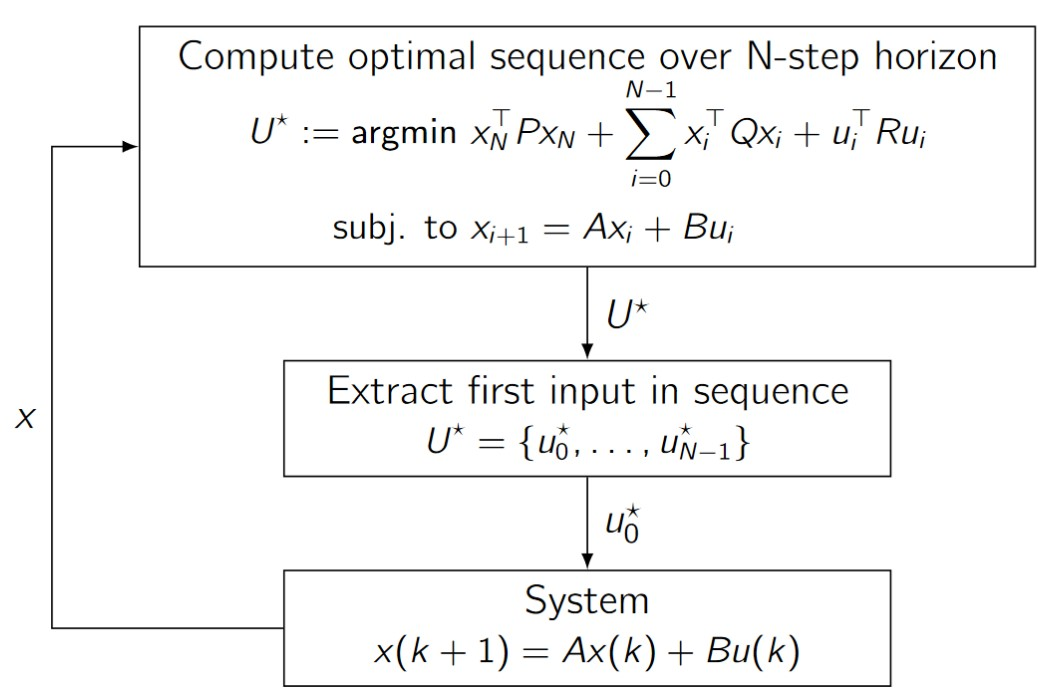
\includegraphics[width = 0.5\linewidth]{MPC_summary/Images/Screenshot 2021-07-31 170253.jpg}
\end{center}

\subsection{Infinite Horizon LQR}
\[\boxed{J_\infty(x(0)) = \sum ^\infty _{i=0}(x_i^TQx_i+ u_i^TRu_i) \mathrm{wth} x_{i+1} = Ax_i+Bu_i}\]
\begin{itemize}
    \item The optimal input is \textbf{time-invariant} (opposed to finite horizon)\[u^*(k) = -(B^TP_\infty B + R )^{-1}B^TP_\infty A x(k) := F_\infty x(k)\]
    \item and the optimal cost approaches: $J_\infty(x(k))=x(k)^TP_\infty X(k)$
    \item if RDE converges to const $P_\infty$ we get: \begin{gather*}P_\infty=A^TP_\infty A + Q \\- A^TP_\infty B(B^TP_\infty B+R)^{-1} B^TP_\infty A\end{gather*}
    \item In fact, if $(A,B)$ stabilizable and $(Q^\frac{1}{2},A)$
 detectable, initialized with $P\infty$ = Q, then the RDE converges to the unique positive definite solution $P_\infty$ of the ARE\end{itemize}


\subsection{Mathematical Optimization Problem}
\begin{gather*}
 \underset{x\in \mathrm{dom}(f)}{\mathrm{min}} f(x)\\
 \mathrm{subj. \hspace{2mm} to. \hspace{2mm} g_i(x) \leq 0 \hspace{2mm} i = 1.,\dots,m}\\
 h_i(x) = 0 \hspace{2mm} i = 1,\dots , p
\end{gather*}
\begin{itemize}
    \item \textbf{Optimization variables} $x:= [x_1, x_2,\dots, x_n]^T]$
    \item \textbf{Objective function:} $f \mathrm{dom}(f) \rightarrow \mathbb{R}$
    \item \textbf{Domain} $\mathrm{dom}(f) \subseteq \mathbb{R}^n$ of the objective $f$
    \item \textbf{Optional inequality} constraint functions \[g_i : \mathbb{R}^n \rightarrow \mathbb{R}, \textrm{for } i =1,\dots,m\]
    \item \textbf{Optional equality} constraint functions \[h_i: \mathbb{R}n \rightarrow \mathbb{R}, \textrm{for } i = 1,\dots, p\]
    \item  \textbf{Feasible set:}
\end{itemize}
    {\small\begin{gather*}\mathcal{X} := \{x\in \textrm{dom}(f) | g_i(x) \leq 0,i=1,\dots,m,\\ h_i(x)=0, i =1,\dots,p \} \end{gather*}}
 \vfill\null\columnbreak
\section{Convex Optimization}
\begin{itemize}
    \item \textbf{Local Optimum:} $x \in \mathcal{X}$ satisfies: $y \in \mathcal{X}. ||y-x|| \leq R \Rightarrow f(y) \geq f(x)$
    \item \textbf{Global Optimum:} $x \in \mathcal{X}$ for some $R > 0: y \in \mathcal{X}. \Rightarrow f(y) \geq f(x)$ 
    \item \textbf{Unbounded:} if $p^* = -\infty$
    \item \textbf{Infeasible:} $\mathcal{X}$ empty $\Leftrightarrow p^* = \infty$
    \item \textbf{Unconstrained:} $\mathcal{X} = \mathbb{R}^n$
\end{itemize}

\subsection{Convex Sets}
A set $\mathcal{X}$ is convex iff for any pair of points $x$ and $y$ in $\mathcal{X}$ can be connected by a line which is always inside the set.
\textbf{mathematical:} \[\lambda x + (1-\lambda) y\in \mathcal{X}, \hspace{4mm} \forall \lambda\in [0,1], \hspace{4mm} \forall x,y \in \mathcal{X} \]
\begin{center}
    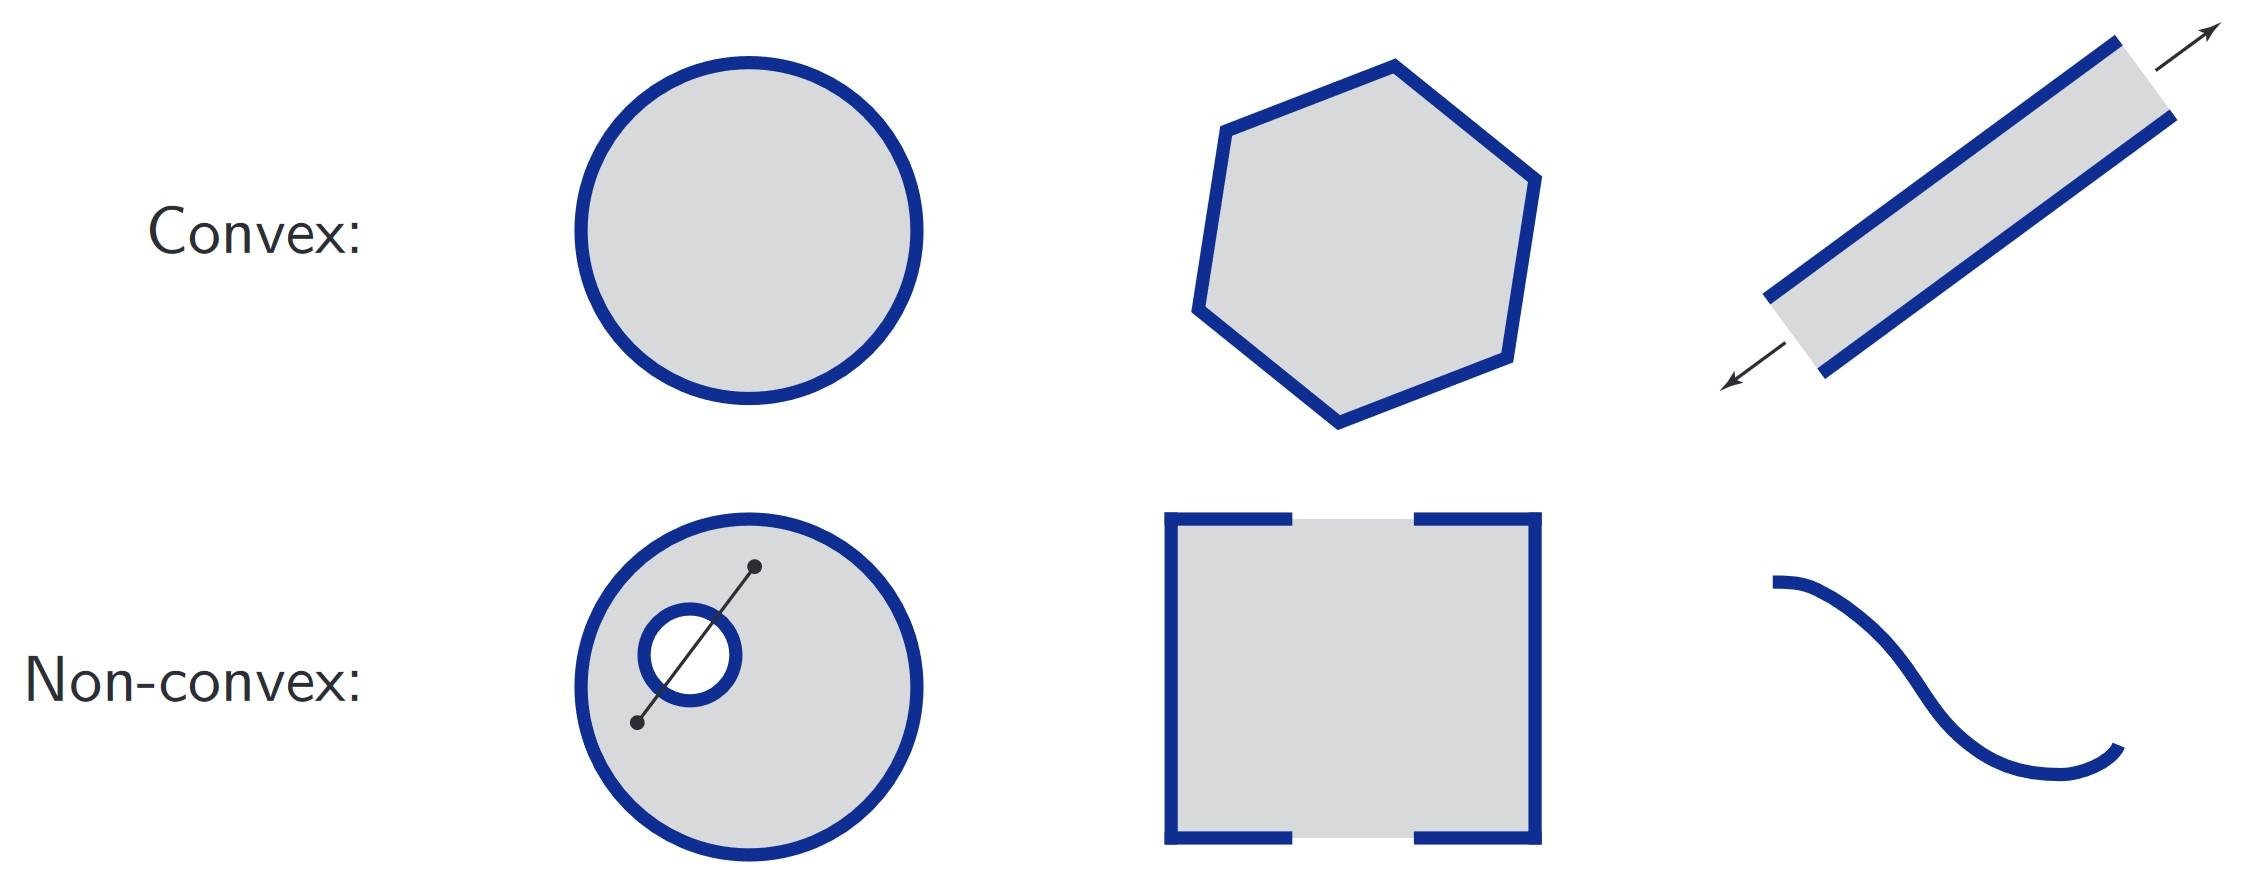
\includegraphics[width= 0.5\linewidth]{MPC_summary/Images/Convex_Non_Convex.jpg}
\end{center}
\subsubsection{Hyperplanes and Halfspaces}
\begin{itemize}
    \item \textbf{Hyperplane} is defined by $\{x\in\mathbb{R}^n| a^Tx = b \}$ for $a \neq 0$ where $a \in \mathcal{R}^n$ is the normal vector to the hyperplane. It is affine and convex.
    \item \textbf{Halfspace} is everything on one side aof a hyperplane $\{x \in \mathbb{R}^n | a^T x \leq b\}$. it can be \textbf{open} (strict inequality) or \textbf{closed} (non-strict inequality). It is convex.
\end{itemize}
\begin{center}
    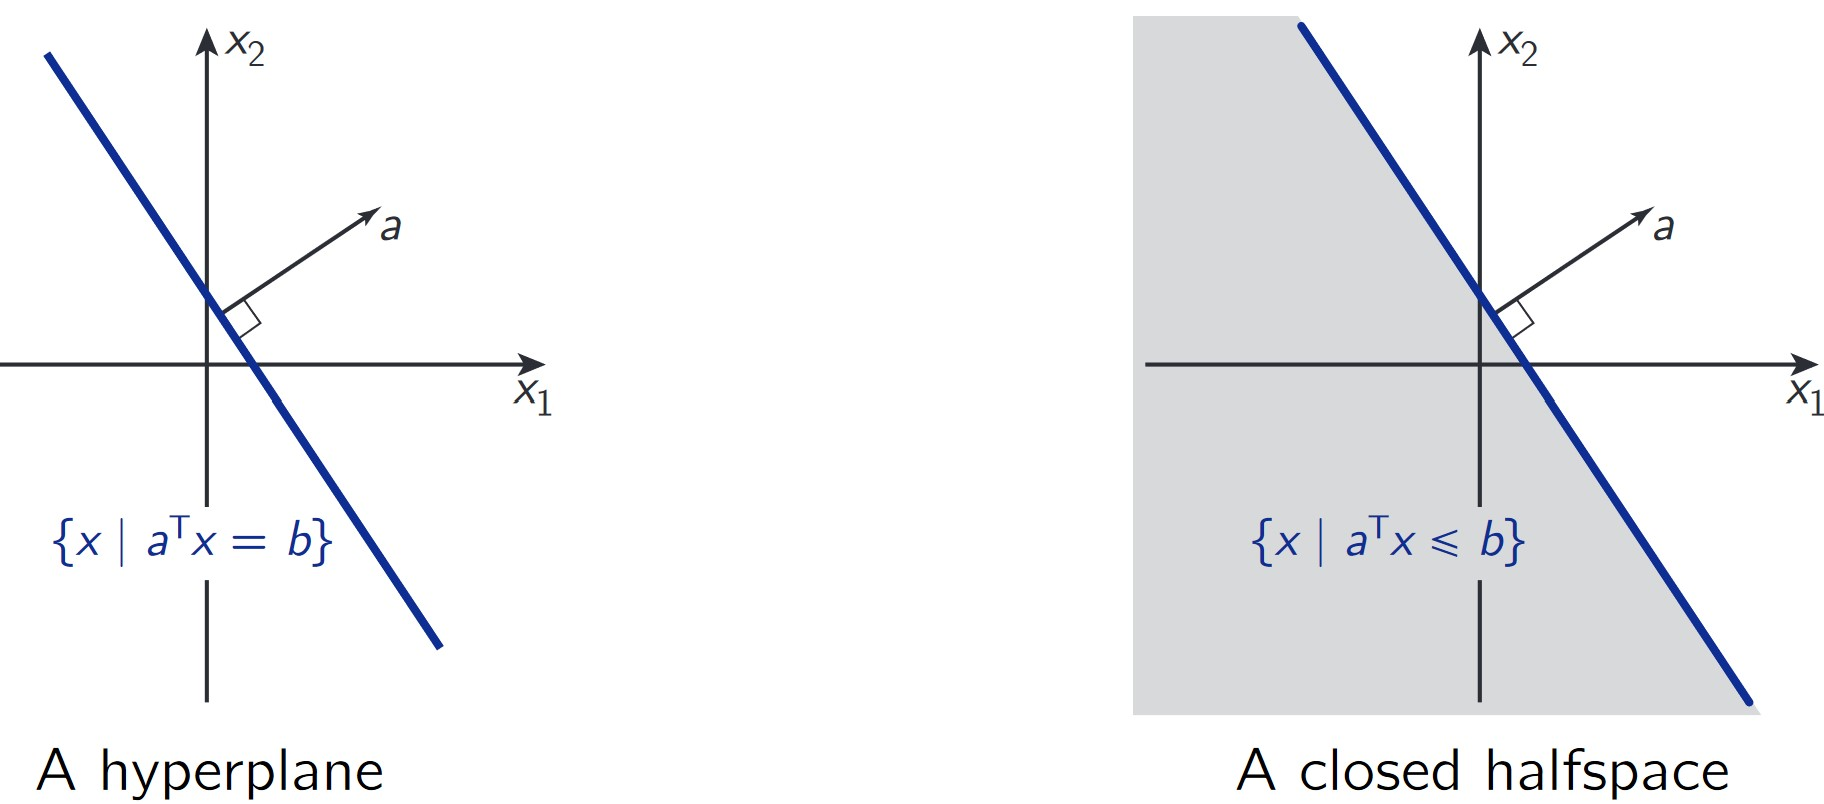
\includegraphics[width= 0.5\linewidth]{MPC_summary/Images/hyperplane_halfspaces.jpg}
\end{center}
\subsubsection{Polyhedra and Polytopes {\tiny(both convex)}}
\begin{itemize}
    \item \textbf{Polyhedron} $:= N \cap$ of closed Halfspaces with $N \in \mathcal{N}$  
    \begin{gather*}P := \{x|a^T_i x \leq b_i,i=1, \dots n\} = \{x|Ax \leq b\}\\
    A := [a_1, \dots a_m]^T,\hspace{3mm} b := [b_1,\dots,b_m]^T
    \end{gather*}
    \item \textbf{Polytope} is a bounded Polyhedron
\end{itemize}
\subsubsection{Ellipsoids}
\begin{itemize}
    \item $\{x|(x-x_c)^T A^{-1}(x-x_c) \leq 1\}$ with  $A\succ 0$ pos. def. and symmetric
\end{itemize}
\subsubsection{Norm Balls}
\begin{itemize}
    \item defined by $\{x|||x-x_c|| \leq r\}$
    \item it is always convex for any norm. 
\end{itemize}
    \begin{gather*}\ell_1: ||x||_1 = \Sigma_i|x_i| \hspace{2mm} \ell_2: ||x||_2 = \sqrt{\Sigma_ix_i^2} \hspace{2mm} \ell_\infty = \underset{i}{max}|x_i|
    \end{gather*}
\subsubsection{Note}
\begin{itemize}
    \item \textbf{intersection} of any convex sets is itself a convex set.
    \item \textbf{union} of two convex sets does not have to be convex.
\end{itemize}
\subsection{Convex Functions}
\textbf{definition: }a function $f$:dom$(f) \rightarrow \mathbb{R}$ is strictly convex iff dom($f$) is convex \textbf{and} $f(\lambda x+(1-\lambda)y) \leq \lambda f(x) + (1-\lambda)f(y), \hspace{2mm} \forall \lambda \in (0,1) \forall x,y \in $ dom($f$)
\begin{itemize}
    \item The function is \textbf{concave} iff dom($f$) is convex and $-f$ is convex
\end{itemize}
\subsubsection{First-Order Condition for Convexity}
\begin{itemize}
    \item A differentiable function $f$ with a convex domain is convex iff
    \begin{gather*}f(y) \geq f(x) + \nabla f(x)^T (y-x), \forall x,y \in \mathrm{dom}(f), \\\nabla f(x) = [\frac{\delta f(x)}{\delta x_1},\dots, \frac{\delta f(x)}{\delta x_n}]^T\end{gather*}
\end{itemize}
\subsubsection{Second-Order Condition for convexity}
\begin{itemize}
    \item A twice differentiable function $f$ with convex domain is convex iff 
    \begin{gather*}
        \nabla ^2 f(x) \succeq 0, \hspace{2mm} \forall x \in \mathrm{dom}(f), \nabla^2f(x)_{ij}=\frac{\delta^2f(x)}{\delta x_i \delta x_j}
    \end{gather*}
\end{itemize}
\subsection{Optimality Conditions}
\subsubsection{Lagrange dual problem}
\textbf{Lagrangian function}
    $\mathbf{L \hspace{2mm}}\mathrm{dom}(f) \times \mathbb{R}^m \times \mathbb{R}^p \rightarrow \mathbb{R}$
\begin{gather*}
    L(x,\lambda,\nu) = f(x) + \sum^m_{i=1} \lambda_i g_i(x)+\sum^p_{i=1}\nu_ih(x)
\end{gather*}
\textbf{Dual function $\mathbf{d}$}
\begin{gather*}
    \mathbf{d}: \mathbb{R}^m\times \mathbb{R}^p: \hspace{5mm} d(\lambda,\nu) = \underset{x\in\mathrm{dom}(f)}{\mathrm{inf}}L(x,\lambda,\nu)
\end{gather*}
\vfill\null\columnbreak
\textbf{NOTE}
\begin{itemize}
    \item dual function is always a \textbf{concave} function
    \item Gradient condition can not be used for a discrete set
\end{itemize}
\subsubsection{Primal (P) Problem}
\begin{gather*}
    \underset{x}{\mathrm{min}}f(x)\\
    \textrm{ sub. to } g_i(x) \leq 0,\hspace{3mm} h_i(x) = 0
\end{gather*}
\subsubsection{Dual (D) Problem}
\begin{gather*}
    \underset{\lambda, \nu}{\mathrm{max}} d(\lambda,\nu)\\
    \textrm{sub. to} \lambda \geq 0
\end{gather*}
\begin{itemize}
    \item Problem (d) is \textbf{convex} even if (P) is not and has optimal value $d^* \leq p^*$
    \item Point $(\lambda ,\nu)$ is \textbf{dual feasible} if $\lambda \geq 0 \textrm{and }(\lambda,\nu) \in dom(f) $ (can be imposed in D)
\end{itemize}
\subsubsection{weak and strong duality}
\textbf{weak}
\begin{itemize}
    \item it is \textbf{always} true that $d^*\leq p^*$
\end{itemize}
\textbf{strong}
\begin{itemize}
    \item it is \textbf{sometimes} true that $d^* = p^*$
    \item Strong duality usually does not hold for non-convex problems.
    \item Can impose conditions on convex problems to guarantee that $d^*= p^*$
    \item Sometimes the dual is much easier to solve than the primal (or vice-versa)
    \item Example: The dual of a mixed integer linear program (difficult to solve) is
a standard LP (easy to solve).
\end{itemize}
\subsubsection{Slater condition}
if $\exists$ \textbf{striclty feasible point} ie.\[ \{ x|Ax= b, g_i(x) < 0 \forall i \in \{1,\dots,m\}\}\neq \emptyset\]
\subsubsection{KKT-Condition}
Assume that $f$, all $g_i$ and $h_i$ are differentiable.
\begin{enumerate}
    \item \textbf{Primal Feasibility:} \begin{gather*}
        g_i(x^*)\leq 0 \hspace{5mm} i = 1,\dots , m\\
        h_i(x^*) = 0 \hspace{5mm} i = 1,\dots, p
    \end{gather*}
    \item \textbf{Dual Feasibility:}
    \begin{gather*}
        \lambda^* \geq 0
    \end{gather*}
    \item\textbf{Complementary Slackness:}
    \begin{gather*}
        \lambda^*_ig_i(x^*) = 0 i = 1,\dots , m 
    \end{gather*}
    \item \textbf{stationarity:}
    \begin{gather*}
        \nabla_xL(x^*, \lambda^*, \nu^*) = \nabla f(x^*) + \sum ^m_{i=1} \lambda_i^*\nabla g_i(x^*) \\+ \sum^p_{i=1} \nu_i^*\nabla h_i (x^*) = 0
    \end{gather*}
\end{enumerate}
\subsubsection{General Optimization: Necessary Condition}
If $x^*$ and ($\lambda^*,\mu^*$) primal and dual sol. (:= zero duality gap ($\epsilon=p^*-d^*$)), then $x^*$ and ($k^*, \mu^*$ satisfy KKT
\subsubsection{Convex Optimization: Necessary and Sufficient Condition}
If $x^*$ and ($\lambda^*, \mu^*$) are primal and dual solutions ($\mathbf{p^* = d^*}$). if \textbf{slater Condition} holds (Strong duality), $x^*$ and ($\lambda^*, \mu^*$) are primal and dual solutions iff they satisfy KKT conditions.
\begin{itemize}
    \item $p^*=f(x^*) = L (x^*,\lambda^*,\mu^*)$ due to Complementary Slackness
    \item $d^* = d(\lambda^*,\mu^*) = L(x^*,\lambda^*,\mu^*)$ due to Convexity of the functions and Stationarity
\end{itemize}

